\documentclass[tikz,10pt]{standalone}
\usepackage{amsmath,amssymb,cmap,pgfplots,pgfplotstable}
\usetikzlibrary{arrows,calc,intersections}
\pgfplotsset{compat=newest}

\begin{document} 
  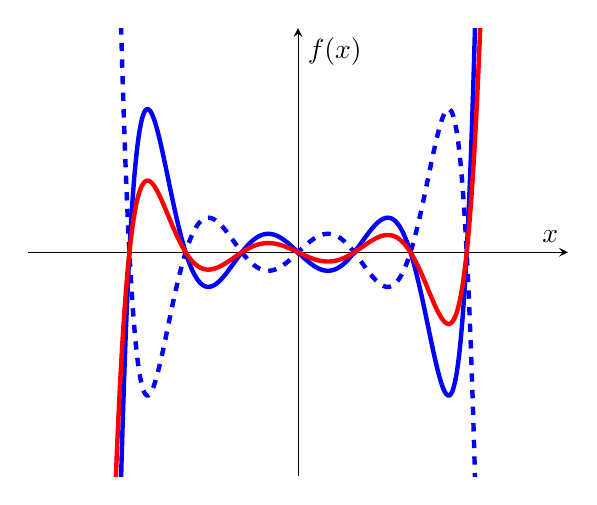
\begin{tikzpicture}
  \begin{axis}[
  xlabel={$x$},
  ylabel={$f(x)$},
  axis lines=middle,
  ymax = 250,
  ymin = -250,
  xmax = 4,
  xmin = -4,
  enlargelimits=true,
  %restrict y to domain=-200:200,
  xtick=\empty,
  ytick=\empty
  ]
  \addplot[
  blue!,
  line width=1.6pt,
  domain={-4:4},
  samples=500
  ]{2*x^7-28*x^5+98*x^3-72*x};
  \addplot[
  blue!,
  dashed,
  line width=1.6pt,
  domain={-4:4},
  samples=500
  ]{-2*x^7+28*x^5-98*x^3+72*x};
  \addplot[
  red!,
  line width=1.6pt,
  domain={-4:4},
  samples=500
  ]{x^7-14*x^5+49*x^3-36*x};
  \end{axis}
  \end{tikzpicture}
\end{document}